\appendix
\chapter{Boxplot graphs}
\label{app:boxplot}

\begin{figure}[H]
\centering
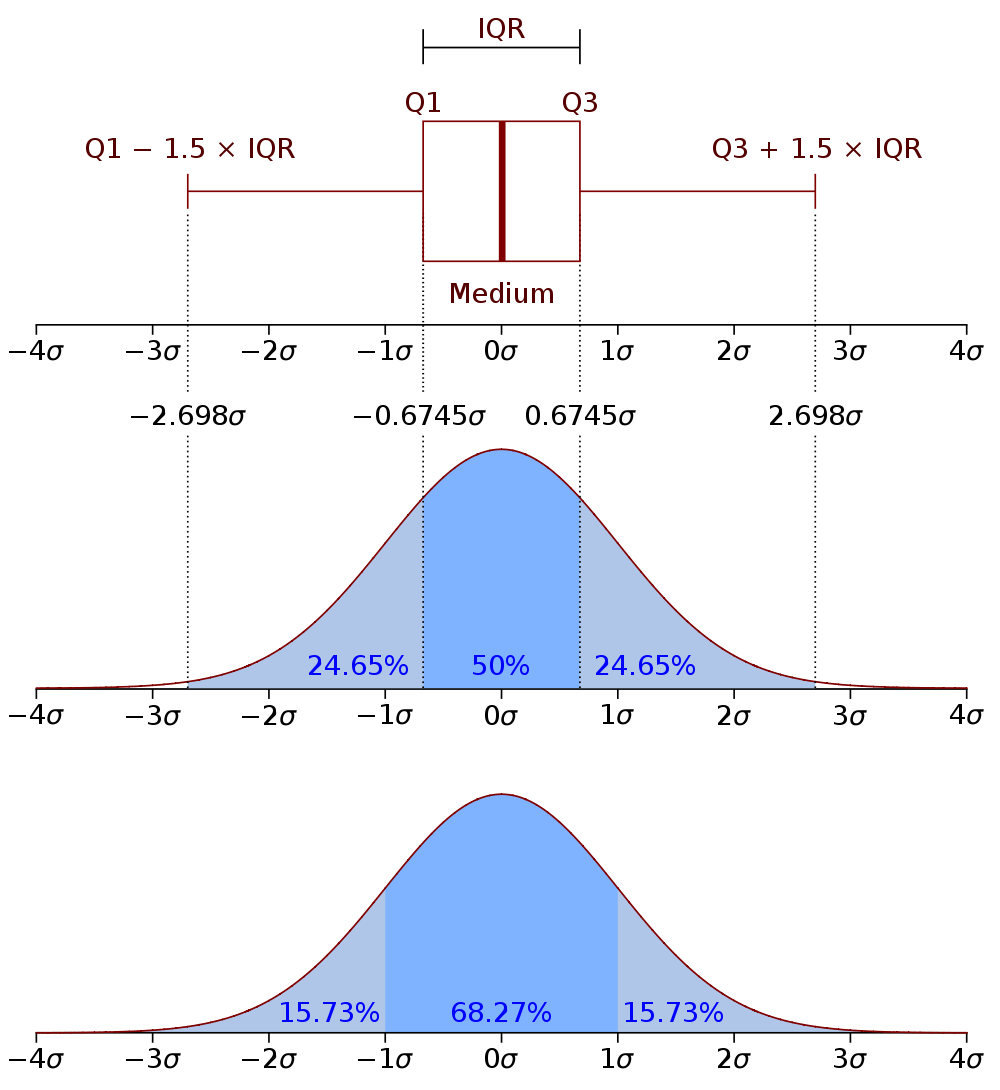
\includegraphics[width=12cm]{boxplot.png}
\caption[How to read a boxplot graph]{How to read a boxplot graph \cite{stk_boxplot}}
\label{boxlot}
\end{figure}

\chapter{SQL scripts}
\section{River assignment}
\label{app:sql_assign_river}

\lstinputlisting[language=SQL, caption={SQL source code for the river assignment process}]{./data/sql_assign_rivers.txt}


\section{Gauge assignment - modeled runoff}
\label{app:sql_assign_watergap}

\lstinputlisting[language=SQL, caption={SQL source code for the runoff assignment process - modeled runoff}]{./data/sql_assign_wg.txt}


\section{Gauge assignment - measured runoff}
\label{app:sql_assign_gauge}

\lstinputlisting[language=SQL, caption={SQL source code for the runoff assignment process - measured runoff}]{./data/sql_assign_gauge.txt}

\chapter{Python scripts of the methods}
\section{Method to get the residual water flow}
\label{app:get_dV_res}

\lstinputlisting[language=python, caption={Python source code for the method fetching the residual water flow}]{./data/python_get_dV_res.txt}

\section{Method to get the nominal water flow}
\label{app:get_dV_n}

\lstinputlisting[language=python, caption={Python source code for the method fetching the nominal water flow}]{./data/python_get_dV_n.txt}

\section{Method to get the type of turbine}
\label{app:get_turb_type}

\lstinputlisting[language=python, caption={Python source code for the method fetching the type of turbine}]{./data/python_get_turb_type.txt}

\section{Computation of the power output}
\label{app:powout}

\lstinputlisting[language=python, caption={Python source code for the functions computing the power output}]{./data/python_power_output.txt}

\chapter{Python scripts of the use examples}

\section{Use example with csv files}
\label{app:ex_with_csv}

\lstinputlisting[language=python, caption={Python script for the use example with csv files}]{./data/python_example_with_csv.txt}

\section{Use example with the OpenEnergy Database}
\label{app:ex_with_oedb}

\lstinputlisting[language=python, caption={Python script for the use example with the OpenEnergy Database}]{./data/python_example_with_oedb.txt}


\chapter{Standard data used in the model}

\section{Table containing the vertices of the turbines characteristic diagrams}
\label{app:csv_vertices}
\begin{table}[H]
\footnotesize
 \centering
 \caption{Vertices of the turbines characteristic diagrams}
 \begin{tabular}{|c|c|c|c|c|c|c|}
 \cline{2-7}
  \multicolumn{1}{c|}{}&Kaplan{\_}dV{\_}n&Kaplan{\_}h{\_}n&Francis{\_}dV{\_}n&Francis{\_}h{\_}n&Pelton{\_}dV{\_}n&Pelton{\_}h{\_}n\\
  \hline
  0&1&2&0.8&10&0.5&120\\
  1&100&2&80&10&30&300\\
  2&1000&20&1000&50&50&1000\\
  3&50&80&1000&100&5&2000\\
  4&10&80&80&800&0.5&2000\\
  5&1&20&5&800&&\\
  6&&&0.8&200&&\\
  \hline
 \end{tabular}
\end{table}

\section{Table containing the parameters to calculate the efficiency of a turbine}
\label{app:csv_eff}
\begin{table}[H]
\footnotesize
 \centering
 \caption{Parameters to calculate the efficiency of a turbine}
 \begin{tabular}{|c|c|c|c|c|c|c|}
 \cline{2-7}
  \multicolumn{1}{c|}{}&type&load{\_}min&eta{\_}n&a1&a2&a3\\
  \hline
0&Kaplan&0.081&0.895&0.045&0.965&0.1\\
1&Pelton&0.07&0.885&0.03&0.99&0.1\\
2&Francis&0.095&0.89&0.18&0.63&0.31\\
3&Propeller&0.42&0.9&0.25&0.28&0.69\\
4&dummy&0.082&0.89&0.085&0.86&0.17\\
  \hline
 \end{tabular}
\end{table}

